\documentclass[12pt]{article}

\usepackage{amsmath, mathtools}
\usepackage{amsfonts}
\usepackage{amssymb}
\usepackage{graphicx}
\usepackage{colortbl}
\usepackage{xr}
\usepackage{hyperref}
\usepackage{longtable}
\usepackage{xfrac}
\usepackage{tabularx}
\usepackage{float}
\usepackage{siunitx}
\usepackage{booktabs}
\usepackage{caption}
\usepackage{pdflscape}
\usepackage{afterpage}

\usepackage[round]{natbib}
\usepackage{helvet}
\usepackage[none]{hyphenat}
\usepackage{tabularx}
\renewcommand{\familydefault}{\sfdefault}

%\usepackage{refcheck}

\hypersetup{
    bookmarks=true,         % show bookmarks bar?
      colorlinks=true,       % false: boxed links; true: colored links
    linkcolor=red,          % color of internal links (change box color with linkbordercolor)
    citecolor=green,        % color of links to bibliography
    filecolor=magenta,      % color of file links
    urlcolor=cyan           % color of external links
}

%% Comments

\usepackage{color}

\newif\ifcomments\commentstrue %displays comments
%\newif\ifcomments\commentsfalse %so that comments do not display

\ifcomments
\newcommand{\authornote}[3]{\textcolor{#1}{[#3 ---#2]}}
\newcommand{\todo}[1]{\textcolor{red}{[TODO: #1]}}
\else
\newcommand{\authornote}[3]{}
\newcommand{\todo}[1]{}
\fi

\newcommand{\wss}[1]{\authornote{blue}{SS}{#1}} 
\newcommand{\plt}[1]{\authornote{magenta}{TPLT}{#1}} %For explanation of the template
\newcommand{\an}[1]{\authornote{cyan}{Author}{#1}}

%% Common Parts

\newcommand{\progname}{ProgName} % PUT YOUR PROGRAM NAME HERE
\newcommand{\authname}{Team \#, Team Name
\\ Student 1 name and macid
\\ Student 2 name and macid
\\ Student 3 name and macid
\\ Student 4 name and macid} % AUTHOR NAMES                  

\usepackage{hyperref}
    \hypersetup{colorlinks=true, linkcolor=blue, citecolor=blue, filecolor=blue,
                urlcolor=blue, unicode=false}
    \urlstyle{same}
                                


% For easy change of table widths
\newcommand{\colZwidth}{1.0\textwidth}
\newcommand{\colAwidth}{0.13\textwidth}
\newcommand{\colBwidth}{0.82\textwidth}
\newcommand{\colCwidth}{0.1\textwidth}
\newcommand{\colDwidth}{0.05\textwidth}
\newcommand{\colEwidth}{0.8\textwidth}
\newcommand{\colFwidth}{0.17\textwidth}
\newcommand{\colGwidth}{0.5\textwidth}
\newcommand{\colHwidth}{0.28\textwidth}

% Used so that cross-references have a meaningful prefix
\newcounter{defnum} %Definition Number
\newcommand{\dthedefnum}{GD\thedefnum}
\newcommand{\dref}[1]{GD\ref{#1}}
\newcounter{datadefnum} %Datadefinition Number
\newcommand{\ddthedatadefnum}{DD\thedatadefnum}
\newcommand{\ddref}[1]{DD\ref{#1}}
\newcounter{theorynum} %Theory Number
\newcommand{\tthetheorynum}{T\thetheorynum}
\newcommand{\tref}[1]{T\ref{#1}}
\newcounter{tablenum} %Table Number
\newcommand{\tbthetablenum}{T\thetablenum}
\newcommand{\tbref}[1]{TB\ref{#1}}
\newcounter{assumpnum} %Assumption Number
\newcommand{\atheassumpnum}{P\theassumpnum}
\newcommand{\aref}[1]{A\ref{#1}}
\newcounter{goalnum} %Goal Number
\newcommand{\gthegoalnum}{P\thegoalnum}
\newcommand{\gsref}[1]{GS\ref{#1}}
\newcounter{instnum} %Instance Number
\newcommand{\itheinstnum}{IM\theinstnum}
\newcommand{\iref}[1]{IM\ref{#1}}
\newcounter{reqnum} %Functional Requirement Number
\newcommand{\frthereqnum}{P\thereqnum}
\newcommand{\frref}[1]{R\ref{#1}}
\newcounter{nfrnum} %NFR Number
\newcommand{\rthenfrnum}{NFR\thenfrnum}
\newcommand{\nfrref}[1]{NFR\ref{#1}}
\newcounter{lcnum} %Likely change number
\newcommand{\lthelcnum}{LC\thelcnum}
\newcommand{\lcref}[1]{LC\ref{#1}}

\usepackage{fullpage}

\newcommand{\deftheory}[9][Not Applicable]
{
\newpage
\noindent \rule{\textwidth}{0.5mm}

\paragraph{RefName: } \textbf{#2} \phantomsection 
\label{#2}

\paragraph{Label:} #3

\noindent \rule{\textwidth}{0.5mm}

\paragraph{Equation:}

#4

\paragraph{Description:}

#5

\paragraph{Notes:}

#6

\paragraph{Source:}

#7

\paragraph{Ref.\ By:}

#8

\paragraph{Preconditions for \hyperref[#2]{#2}:}
\label{#2_precond}

#9

\paragraph{Derivation for \hyperref[#2]{#2}:}
\label{#2_deriv}

#1

\noindent \rule{\textwidth}{0.5mm}

}

\begin{document}

\title{Software Requirements Specification for \progname: subtitle describing software} 
\author{\authname}
\date{\today}
	
\maketitle

~\newpage

\pagenumbering{roman}

\tableofcontents

~\newpage

\section*{Revision History}

\begin{tabularx}{\textwidth}{p{3cm}p{2cm}X}
\toprule {\bf Date} & {\bf Version} & {\bf Notes}\\
\midrule
Date 1 & 1.0 & Notes\\
Date 2 & 1.1 & Notes\\
\bottomrule
\end{tabularx}

~\newpage

\section{Reference Material}

This section records information for easy reference.

\subsection{Table of Units}

Throughout this document SI (Syst\`{e}me International d'Unit\'{e}s) is employed
as the unit system.  In addition to the basic units, several derived units are
used as described below.  For each unit, the symbol is given followed by a
description of the unit and the SI name.
~\newline

\renewcommand{\arraystretch}{1.2}
%\begin{table}[ht]
  \noindent \begin{tabular}{l l l} 
    \toprule		
    \textbf{symbol} & \textbf{unit} & \textbf{SI}\\
    \midrule 
    \si{\metre} & length & metre\\
    \si{\kilogram} & mass	& kilogram\\
    \si{\second} & time & second\\
    \si{\degree} & angle & degree\\
    \si{\radian} & angle & radian\\
    \si{\V} & potential & volts\\
    \si{\ampere} & current & ampere\\
    \si{\ohm} & resistance & ohm (\si\ohm = \si{\V\per\ampere})\\
    \si{\F} & capacitance & farad\\
    \si{\H} & inductance & henry\\
    N & force & newton (N = \si{\kilogram\metre\per\square\second})\\
    Pa & pressure & pascals (Pa = N\si{\per\square\metre})\\
    \si{\Hz} & frequency & hertz\\
    \si{\joule} & energy & joule\\
    \si{\watt} & power & watt (W = \si{\joule\per\second})\\
    \bottomrule
  \end{tabular}
  
  ~\newline
Below are some derived units that do not use a specific SI symbol.
~\newline

  \renewcommand{\arraystretch}{1.2}
%\begin{table}[ht]
  \noindent \begin{tabular}{l l} 
    \toprule		
    \textbf{Derived unit} & \textbf{SI}\\
    \midrule 
    area  & \si{\square\metre}\\
    volume & \si{\cubic\metre}\\
    velocity &  \si{\metre\per\second}\\
    acceleration &  \si{\metre\per\square\second}\\    
    \bottomrule
  \end{tabular}
  
  %	\caption{Provide a caption}
%\end{table}


\subsection{Table of Symbols}

The table that follows summarizes the symbols used in this document along with
their units.  The choice of symbols was made to be consistent with kinematics and existing documentation of existing activity trackers. The symbols are listed in alphabetical order.

\renewcommand{\arraystretch}{1.2}
%\noindent \begin{tabularx}{1.0\textwidth}{l l X}
\noindent \begin{longtable*}{l l p{12cm}} \toprule
\textbf{symbol} & \textbf{unit} & \textbf{description}\\
\midrule
$f_c$ & \si{\Hz} & clock frequency of microcontroller\\
$m_{tracker}$ & \si\g & mass of activity tracker (device)\\
$a_r$ & \si{\metre\per\square\second} & accelerometer resolution\\
$A_{tracker}$ & \si[per-mode=symbol] {\square\metre} & estimated area of activity tracker\\
$V_{battery}$ & \si\V & supplied voltage of battery\\

\bottomrule
\end{longtable*}

\subsection{Abbreviations and Acronyms}

\renewcommand{\arraystretch}{1.2}
\begin{tabular}{l l} 
  \toprule		
  \textbf{symbol} & \textbf{description}\\
  \midrule 
  A & Assumption\\
  ACC & Acceleration\\
  BAR & Barometer\\
  CSV & Comma-Separated Values\\
  CV & Controlled Variables\\
  DD & Data Definition\\
  EMA & Ecological Momentary Assessment\\
  FSM & Finite State Machine\\
  GD & General Definition\\
  GS & Goal Statement\\
  GYR & Gyrometer\\
  IM & Instance Model\\
  LC & Likely Change\\
  LSS & Lumbar Spinal Stenosis\\
  MV & Monitored Variables\\
  NFR & Non-Functional Requirements\\
  OOP & Object Oriented Programming\\
  PID & Proportional-integral-derivative\\
  PS & Physical System Description\\
  R & Requirement\\
  SI & Syst\`{e}me International d'Unit\'{e}s\\
  SReS & School of Rehabilitation Sciences\\
  SRS & Software Requirements Specification\\
  \bottomrule
\end{tabular}\\

\subsection{Mathematical Notation}
N/A
\pagenumbering{arabic}

\section{Introduction}

Researchers at the School of Rehabilitation Sciences (SReS) at McMaster University are investigating treatment strategies for victims of spinal disorders and back pain. Currently, there is great interest in performing Ecological Momentary Assessment (EMA) of those who suffer from back pain and disorders in order to make treatment options more effective. EMA aims to study the thoughts, experiences, and behaviours of a patient's daily life by repeatedly collecting data in an individual's normal environment, at or close to the time they carry out that behaviour.\\

Specifically, the type of EMA that the SReS is interested in is focused on analyzing the daily activities and symptoms of mostly-older adults with mobility and spinal issues. For example, they may be interested in performing EMA on a patient with spinal compression issues which prevent them from being able to walk long distances without experiencing pain or distress. They wish to track that patient's walking activity as they go about their daily life. If this patient stops walking or moving, they wish to prompt them with questions such as, "Did you stop moving? If so, was it due to pain? Describe your pain, describe which portion of the body it is in." The answers to these questions will be combined with activity monitoring data to form a better picture about the experience this patient has with their spinal and mobility issues.\\

In order to accomplish this, the researchers have attempted to use various smart-watch-esque activity tracking devices to track the activity of their patients, and have attempted to use apps and different pieces of software for them to prompt their patients with questions. However, they have been frustrated with very limited success, and are looking for a system which integrated precise and relevant activity tracking with user-friendly self-reporting symptom functionality.\\

The researchers require a method to perform EMA analysis in a manner which even older patients can use, integrated into one package which gathers relevant data about a patient's activities and allows them to easily report what is currently going on and how they feel. They also are looking for a way to access EMA data in various ways. This includes graphical representations of the data which are meaningful to researchers, along with the raw data itself. This data could be activity data, symptoms reporting data, both types of data collated together, and so on. \\

This introductory section of the document is intended to provide a reader with an overview of the purpose, overall scope, and organization of the document. As well as a description of the characteristics of the intended reader of this document.\\

\subsection{Purpose of Document}

This document is intended to describe the requirements of Team \#1's system in a structured and collected manner. In other words, this is a document focused on what the system needs to do and the metrics and methods used to measure its performance. This groundwork is laid in a way to allow every individual who reads this document to understand the details essential to the requirements of this system.\\

Additional purposes of this document are to plan for the design stage of the project, foster effective communication between members of the team, and to establish reference material to which team members will be able to refer back to at later stages in the project should they need to acquire a higher-level view of the system.

\subsection{Scope of Requirements} 

The scope requirements for a system which satisfies the goals of EMA must be defined properly. In the case of this project, the requirements must include a method of activity monitoring and a way to prompt users with questions relevant to EMA. In addition, this system will be used by older adults in Canada, specifically in a typical Canadian household environment, likely with a fixed daily routine. This system is not intended to be used by bedridden or sedentary users. If a user is unable to maintain a certain level of movement on a regular basis, the entire point of EMA is rendered moot. It is also necessary to exclude children from the sphere of users. This system must be designed for adults, aimed specifically towards older adults.\\

\subsection{Characteristics of Intended Reader} \label{sec_IntendedReader}

While this document is intended to describe the requirements of the system in as abstract of a method as possible, it is unreasonable to expect a layman without any knowledge within the field of mechatronics to understand the contents of this document. Therefore, there are certain characteristics that a reader must have in order to fully grasp the scope of this SRS. \\

A reader should have a grasp of software development, electronics, mechanics and dynamics at a level equivalent to a 3rd-Year Mechatronics Undergraduate University student, as well as a basic understanding of human anatomy of which a high school level is adequate. \\

In addition, a reader should have a high-level understanding of Ecological Momentary Assessment. This does not have to be particularly in depth, but a reader should be able to identify the main objectives, practices, and difficulties of performing EMA. Introductory resources related to this can be found here [specify where]. \\

\subsection{Organization of Document}
I'm leaving this section until we finalize section 5 and beyond. It won't take long. -JH\\

\plt{This section provides a roadmap of the SRS document.  It will help the
  reader orient themselves.  It will provide direction that will help them
  select which sections they want to read, and in what order.  This section will
  be similar between project.}

\section{General System Description}

This section provides general information about the system.  It identifies the
interfaces between the system and its environment, describes the user
characteristi	cs and lists the system constraints.  \\\\
\subsection{System Context}

This system in theory is very simple. An array of sensors grabs info regarding the position, speed, orientation, etc. and uses that information to understand the current state of the user. This data is then used to generate prompts that the user will answer and all the collected data is compiled, processed and stored within the system. Finally, researchers will analyze the collected data and generate observations. 
\begin{figure}[h!]
\begin{center}
 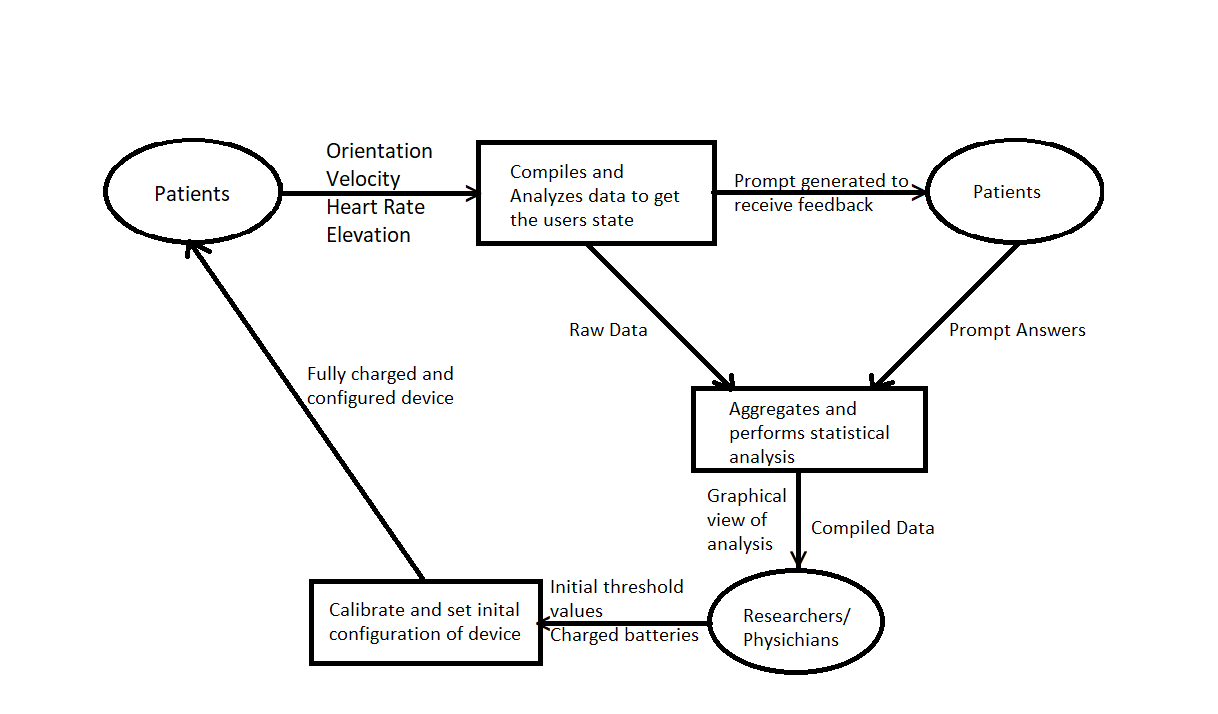
\includegraphics[width=.95\textwidth]{System Context Diagram}
\caption{System Context}
\label{Fig_SystemContext} 
\end{center}
\end{figure}

The design has 2 different users:
\begin{itemize}
\item \textbf{Researchers}: Primary end user who will use the data collected by the device for analysis and research.
\item \textbf{Patients} : Users part of the monitoring study who will be wearing the device, and whose activities will be collected for research and analysis.

\end{itemize}

\begin{itemize}
\item Patient Responsibilities:
\begin{itemize}
\item Patients are required to set up the device correctly so that their various attributes (Orientation, velocity, etc.) can be collected.
\item Patients are also required to answer the prompts given to them so that adequate data can be collected.
\end{itemize}
\item Researcher Responsibilities:
\begin{itemize}
\item Required to confirm that data is being collected.
\item Required to set up the intial thresholds and activities for tracking.
\item Offshoot the data.
\item Charge and calibrate the system.
\end{itemize}
\end{itemize}

\subsection{User Characteristics} \label{SecUserCharacteristics}

Patients should have a general understanding of using smart devices with touch screen interfaces. Patients will also be required to wear the device on their body so a good understanding of how to setup the device and secure it will be required. Finally the device will prompt users to answer certain prompts, thus knowledge of what to expect and how to respond is required.\\

Researchers will have the option of tweaking the configuration of the device, allowing them to manipulate certain activity thresholds. Thus a working knowledge of the system is required. Moreover, a basic understanding of graphs andd statistical analysis will be required to understand the research data collected by the device.\\\\


\subsection{System Constraints}

The design will consist of both a hardware and a software system. The constraints for both systems are as follows:
\begin{itemize}
\item \textbf{Hardware}: 
	\begin{itemize}
		\item The system must weigh less than 60g to facilitate being lightweight and comfortable.
		\item The system must have an average battery life of atleast 7 days to facilitate monitoring of the users.
		\item The dimensions of the system must be quite small with an area lower than 2500mm\textsuperscript{2}.\\
	\end{itemize}

\item \textbf{Software} :
	\begin{itemize}
		\item The system will have hard time constrainsts so as to store data and prompt users with low latency .
		\item To maintain privacy, the system will only store data for two weeks after which the data will be deleted.
		\item The system must prompt users based on activities and not based on time of day. 
	\end{itemize}
\end{itemize}


\section{Specific System Description}

This section first presents the problem description, which gives a high-level
view of the problem to be solved.  This is followed by the solution characteristics
specification, which presents the assumptions, theories, definitions and finally
the instance models.  \plt{Add any project specific details that are relevant
  for the section overview.}

\subsection{Problem Description} \label{Sec_pd}

\progname{} is intended to solve ... \plt{What problem does your program solve?
The description here should be in the problem space, not the solution space.}

\subsubsection{Terminology and  Definitions}

This subsection provides a list of terms that are used in the subsequent
sections and their meaning, with the purpose of reducing ambiguity and making it
easier to correctly understand the requirements:

\begin{itemize}

\item 

\end{itemize}

\subsubsection{Physical System Description} \label{sec_phySystDescrip}

\plt{The purpose of this section is to clearly and unambiguously state the
  physical system that is to be modelled. Effective problem solving requires a
  logical and organized approach. The statements on the physical system to be
  studied should cover enough information to solve the problem. The physical
  description involves element identification, where elements are defined as
  independent and separable items of the physical system. Some example elements
  include acceleration due to gravity, the mass of an object, and the size and
  shape of an object. Each element should be identified and labelled, with their
  interesting properties specified clearly. The physical description can also
  include interactions of the elements, such as the following: i) the
  interactions between the elements and their physical environment; ii) the
  interactions between elements; and, iii) the initial or boundary conditions.}

The physical system of \progname{}, as shown in Figure~?,
includes the following elements:

\begin{itemize}

\item[PS1:] 

\item[PS2:] ...

\end{itemize}

\plt{A figure here makes sense for most SRS documents}

% \begin{figure}[h!]
% \begin{center}
% %\rotatebox{-90}
% {
%  \includegraphics[width=0.5\textwidth]{<FigureName>}
% }
% \caption{\label{<Label>} <Caption>}
% \end{center}
% \end{figure}

\subsubsection{Goal Statements}

\plt{The goal statements refine the ``Problem Description''
  (Section~\ref{Sec_pd}).  A goal is a functional objective the system under
  consideration should achieve. Goals provide criteria for sufficient
  completeness of a requirements specification and for requirements
  pertinence. Goals will be refined in Section “Instanced Models”
  (Section~\ref{sec_instance}). Large and complex goals should be decomposed
  into smaller sub-goals.  The goals are written abstractly, with a minimal
  amount of technical language.  They should be understandable by non-domain
  experts.}

\noindent Given the \plt{inputs}, the goal statements are:

\begin{itemize}

\item[GS\refstepcounter{goalnum}\thegoalnum \label{G_meaningfulLabel}:] \plt{One
    sentence description of the goal.  There may be more than one.  Each Goal
    should have a meaningful label.}

\end{itemize}

\subsection{Solution Characteristics Specification}

\plt{This section specifies the information in the solution domain of the system
  to be developed. This section is intended to express what is required in
  such a way that analysts and stakeholders get a clear picture, and the
  latter will accept it. The purpose of this section is to reduce the problem
  into one expressed in mathematical terms. Mathematical expertise is used to
  extract the essentials from the underlying physical description of the
  problem, and to collect and substantiate all physical data pertinent to the
  problem.}

\plt{This section presents the solution characteristics by successively refining
  models.  It starts with the abstract/general Theoretical Models (TMs) and
  refines them to the concrete/specific Instance Models (IMs).  If necessary
  there are intermediate refinements to General Definitions (GDs).  All of these
  refinements can potentially use Assumptions (A) and Data Definitions (DD).
  TMs are refined to create new models, that are called GMs or IMs. DDs are not
  refined; they are just used. GDs and IMs are derived, or refined, from other
  models. DDs are not derived; they are just given. TMs are also just given, but
  they are refined, not used.  If a potential DD includes a derivation, then
  that means it is refining other models, which would make it a GD or an IM.}

\plt{The above makes a distinction between ``refined'' and ``used.'' A model is
  refined to another model if it is changed by the refinement. When we change a
  general 3D equation to a 2D equation, we are making a refinement, by applying
  the assumption that the third dimension does not matter. If we use a
  definition, like the definition of density, we aren't refining, or changing
  that definition, we are just using it.}

\plt{The same information can be a TM in one problem and a DD in another.  It is
  about how the information is used.  In one problem the definition of
  acceleration can be a TM, in another it would be a DD.}

\plt{There is repetition between the information given in the different chunks
  (TM, GDs etc) with other information in the document.  For instance, the
  meaning of the symbols, the units etc are repeated.  This is so that the
  chunks can stand on their own when being read by a reviewer/user.  It also
  facilitates reuse of the models in a different context.}

\noindent \plt{The relationships between the parts of the document are show in
  the following figure.  In this diagram ``may ref'' has the same role as
  ``uses'' above.  The figure adds ``Likely Changes,'' which are able to
  reference (use) Assumptions.}

\begin{figure}[H]
  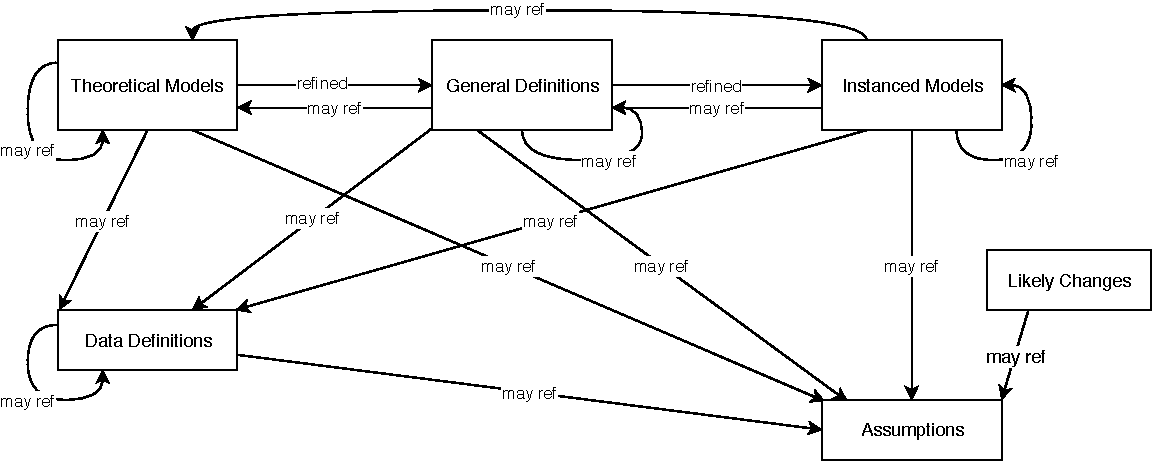
\includegraphics[scale=0.9]{RelationsBetweenTM_GD_IM_DD_A.pdf}
\end{figure}

The instance models that govern \progname{} are presented in
Subsection~\ref{sec_instance}.  The information to understand the meaning of the
instance models and their derivation is also presented, so that the instance
models can be verified.

\subsubsection{Assumptions} \label{sec_assumpt}

\plt{The assumptions are a refinement of the scope.  The scope is general, where
  the assumptions are specific.  All assumptions should be listed, even those
  that domain experts know so well that they are rarely (if ever) written down.}
\plt{The document should not take for granted that the reader knows which
  assumptions have been made. In the case of unusual assumptions, it is
  recommended that the documentation either include, or point to, an explanation
  and justification for the assumption.}

This section simplifies the original problem and helps in developing the
theoretical model by filling in the missing information for the physical
system. The numbers given in the square brackets refer to the theoretical model
[T], general definition [GD], data definition [DD], instance model [IM], or
likely change [LC], in which the respective assumption is used.

\begin{itemize}

\item[A\refstepcounter{assumpnum}\theassumpnum
\label{A1}:]
{All users are fluent English speakers.}

\item[A\refstepcounter{assumpnum}\theassumpnum
\label{A2}:]
{The device is to be used under normal daily activities.}

\item[A\refstepcounter{assumpnum}\theassumpnum
\label{A3}:]
{The device does not have to receive or send data in any wireless manner. It will only have to transfer data through wired connections.}

\item[A\refstepcounter{assumpnum}\theassumpnum
\label{A4}:]
{All patients are to receive verbal instructions from their researcher on how to use their devices.}

\end{itemize}

\subsubsection{Theoretical Models}\label{sec_theoretical}

\plt{Theoretical models are sets of abstract mathematical equations or axioms
  for solving the problem described in Section ``Physical System Description''
  (Section~\ref{sec_phySystDescrip}). Examples of theoretical models are
  physical laws, constitutive equations, relevant conversion factors, etc.}

This section focuses on the general equations and laws that \progname{} is based
on.  \plt{Modify the examples below for your problem, and add additional models
  as appropriate.}

~\newline

\noindent
\deftheory
% #2 refname of theory
{T:COE}
% #3 label
{Conservation of thermal energy}
% #4 equation
{
  $-{\bf \nabla \cdot q} + g$ = $\rho C \frac{\partial T}{\partial t}$
}
% #5 description
{
  The above equation gives the conservation of energy for transient heat transfer in a material
  of specific heat capacity $C$ (\si{\joule\per\kilogram\per\celsius}) and density $\rho$ 
  (\si{\kilogram\per\cubic\metre}), where $\bf q$ is the thermal flux vector (\si{\watt\per\square\metre}),
  $g$ is the volumetric heat generation
  (\si{\watt\per\cubic\metre}), $T$ is the temperature
  (\si{\celsius}),  $t$ is time (\si{\second}), and $\nabla$ is
  the gradient operator.  For this equation to apply, other forms
  of energy, such as mechanical energy, are assumed to be negligible in the
  system (\aref{A_OnlyThermalEnergy}).  In general, the material properties ($\rho$ and $C$) depend on temperature.
}
% #6 Notes
{
None.
}
% #7 Source
{
  \url{http://www.efunda.com/formulae/heat_transfer/conduction/overview_cond.cfm}
}
% #8 Referenced by
{
  \dref{ROCT}
}
% #9 Preconditions
{
None
}
% #1 derivation - not applicable by default
{}

\plt{``Ref.\ By'' is used repeatedly with the different types of information.
  This stands for Referenced By.  It means that the models, definitions and
  assumptions listed reference the current model, definition or assumption.
  This information is given for traceability.  Ref. By provides a pointer in the
  opposite direction to what we commonly do.  You still need to have a reference
  in the other direction pointing to the current model, definition or
  assumption.  As an example, if T1 is referenced by G2, that means that G2 will
  explicitly include a reference to T1.}

~\newline

\subsubsection{General Definitions}\label{sec_gendef}

\plt{General Definitions (GDs) are a refinement of one or more TMs, and/or of
  other GDs.  The GDs are less abstract than the TMs.  Generally the reduction
  in abstraction is possible through invoking (using/referencing) Assumptions.
  For instance, the TM could be Newton's Law of Cooling stated abstracting.  The
  GD could take the general law and apply it to get a 1D equation.}

This section collects the laws and equations that will be used in building the
instance models.

\plt{Some projects may not have any content for this section, but the section
  heading should be kept.}  \plt{Modify the examples below for your problem, and
  add additional definitions as appropriate.}

~\newline

\noindent
\begin{minipage}{\textwidth}
\renewcommand*{\arraystretch}{1.5}
\begin{tabular}{| p{\colAwidth} | p{\colBwidth}|}
\hline
\rowcolor[gray]{0.9}
Number& GD\refstepcounter{defnum}\thedefnum \label{NL}\\
\hline
Label &\bf Newton's law of cooling \\
\hline
% Units&$MLt^{-3}T^0$\\
% \hline
SI Units&\si{\watt\per\square\metre}\\
\hline
Equation&$ q(t) = h \Delta T(t)$  \\
\hline
Description &
Newton's law of cooling describes convective cooling from a surface.  The law is
stated as: the rate of heat loss from a body is proportional to the difference
in temperatures between the body and its surroundings.
\\
& $q(t)$ is the thermal flux (\si{\watt\per\square\metre}).\\
& $h$ is the heat transfer coefficient, assumed independent of $T$ (\aref{A_hcoeff})
	(\si{\watt\per\square\metre\per\celsius}).\\
&$\Delta T(t)$= $T(t) - T_{\text{env}}(t)$ is the time-dependent thermal gradient
between the environment and the object (\si{\celsius}).
\\
\hline
  Source & Citation here \\
  \hline
  Ref.\ By & \ddref{FluxCoil}, \ddref{FluxPCM}\\
  \hline
\end{tabular}
\end{minipage}\\

\subsubsection*{Detailed derivation of simplified rate of change of temperature}

\plt{This may be necessary when the necessary information does not fit in the
  description field.}
\plt{Derivations are important for justifying a given GD.  You want it to be
  clear where the equation came from.}

\subsubsection{Data Definitions}\label{sec_datadef}

\plt{The Data Definitions are definitions of symbols and equations that are
  given for the problem.  They are not derived; they are simply used by other
  models.  For instance, if a problem depends on density, there may be a data
  definition for the equation defining density.  The DDs are given information
  that you can use in your other modules.}

\plt{All Data Definitions should be used (referenced) by at least one other
  model.}

This section collects and defines all the data needed to build the instance
models. The dimension of each quantity is also given.  \plt{Modify the examples
  below for your problem, and add additional definitions as appropriate.}

~\newline

\noindent
\begin{minipage}{\textwidth}
\renewcommand*{\arraystretch}{1.5}
\begin{tabular}{| p{\colAwidth} | p{\colBwidth}|}
\hline
\rowcolor[gray]{0.9}
Number& DD\refstepcounter{datadefnum}\thedatadefnum \label{FluxCoil}\\
\hline
Label& \bf Heat flux out of coil\\
\hline
Symbol &$q_C$\\
\hline
% Units& $Mt^{-3}$\\
% \hline
  SI Units & \si{\watt\per\square\metre}\\
  \hline
  Equation&$q_C(t) = h_C (T_C - T_W(t))$, over area $A_C$\\
  \hline
  Description & 
                $T_C$ is the temperature of the coil (\si{\celsius}).  $T_W$ is the temperature of the water (\si{\celsius}).  
                The heat flux out of the coil, $q_C$ (\si{\watt\per\square\metre}), is found by
                assuming that Newton's Law 
                of Cooling applies (\aref{A_Newt_coil}).  This law (\dref{NL}) is used on the surface of
                the coil, which has area $A_C$ (\si{\square\metre}) and heat 
                transfer coefficient $h_C$
                (\si{\watt\per\square\metre\per\celsius}).  This equation
                assumes that the temperature of the coil is constant over time (\aref{A_tcoil}) and that it does not vary along the length
                of the coil (\aref{A_tlcoil}).
  \\
  \hline
  Sources& Citation here \\
  \hline
  Ref.\ By & \iref{ewat}\\
  \hline
\end{tabular}
\end{minipage}\\

\subsubsection{Data Types}\label{sec_datatypes}

\plt{This section is optional.  In many scientific computing programs it isn't
  necessary, since the inputs and outpus are straightforward types, like reals,
  integers, and sequences of reals and integers.  However, for some problems it
  is very helpful to capture the type information.}

\plt{The data types are not derived; they are simply stated and used by other
  models.}

\plt{All data types must be used by at least one of the models.}

\plt{For the mathematical notation for expressing types, the recommendation is
  to use the notation of~\citet{HoffmanAndStrooper1995}.}

This section collects and defines all the data types needed to document the
models. \plt{Modify the examples below for your problem, and add additional
  definitions as appropriate.}

~\newline

\noindent
\begin{minipage}{\textwidth}
\renewcommand*{\arraystretch}{1.5}
\begin{tabular}{| p{\colAwidth} | p{\colBwidth}|}
  \hline
  \rowcolor[gray]{0.9}
  Type Name & Name for Type\\
  \hline
  Type Def & mathematical definition of the type\\
  \hline
  Description & description here
  \\
  \hline
  Sources & Citation here, if the type is borrowed from another source\\
  \hline
\end{tabular}
\end{minipage}\\

\subsubsection{Instance Models} \label{sec_instance}    

\plt{The motivation for this section is to reduce the problem defined in
  ``Physical System Description'' (Section~\ref{sec_phySystDescrip}) to one
  expressed in mathematical terms. The IMs are built by refining the TMs and/or
  GDs.  This section should remain abstract.  The SRS should specify the
  requirements without considering the implementation.}

This section transforms the problem defined in Section~\ref{Sec_pd} into 
one which is expressed in mathematical terms. It uses concrete symbols defined 
in Section~\ref{sec_datadef} to replace the abstract symbols in the models 
identified in Sections~\ref{sec_theoretical} and~\ref{sec_gendef}.

The goals \plt{reference your goals} are solved by \plt{reference your instance
  models}.  \plt{other details, with cross-references where appropriate.}
\plt{Modify the examples below for your problem, and add additional models as
  appropriate.}

~\newline

%Instance Model 1

\noindent
\begin{minipage}{\textwidth}
\renewcommand*{\arraystretch}{1.5}
\begin{tabular}{| p{\colAwidth} | p{\colBwidth}|}
  \hline
  \rowcolor[gray]{0.9}
  Number& IM\refstepcounter{instnum}\theinstnum \label{ewat}\\
  \hline
  Label& \bf Energy balance on water to find $T_W$\\
  \hline
  Input&$m_W$, $C_W$, $h_C$, $A_C$, $h_P$, $A_P$, $t_\text{final}$, $T_C$, 
  $T_\text{init}$, $T_P(t)$ from \iref{epcm}\\
  & The input is constrained so that $T_\text{init} \leq T_C$ (\aref{A_charge})\\
  \hline
  Output&$T_W(t)$, $0\leq t \leq t_\text{final}$, such that\\
  &$\frac{dT_W}{dt} = \frac{1}{\tau_W}[(T_C - T_W(t)) + {\eta}(T_P(t) - T_W(t))]$,\\
  &$T_W(0) = T_P(0) = T_\text{init}$ (\aref{A_InitTemp}) and $T_P(t)$ from \iref{epcm} \\
  \hline
  Description&$T_W$ is the water temperature (\si{\celsius}).\\
  &$T_P$ is the PCM temperature (\si{\celsius}).\\
  &$T_C$ is the coil temperature (\si{\celsius}).\\
  &$\tau_W = \frac{m_W C_W}{h_C A_C}$ is a constant (\si{\second}).\\
  &$\eta = \frac{h_P A_P}{h_C A_C}$ is a constant (dimensionless).\\
  & The above equation applies as long as the water is in liquid form,
  $0<T_W<100^o\text{C}$, where $0^o\text{C}$ and $100^o\text{C}$ are the melting
  and boiling points of water, respectively (\aref{A_OpRange}, \aref{A_Pressure}).
  \\
  \hline
  Sources& Citation here \\
  \hline
  Ref.\ By & \iref{epcm}\\
  \hline
\end{tabular}
\end{minipage}\\

%~\newline

\subsubsection*{Derivation of ...}

\plt{The derivation shows how the IM is derived from the TMs/GDs.  In cases
  where the derivation cannot be described under the Description field, it will
  be necessary to include this subsection.}

\subsubsection{Input Data Constraints} \label{sec_DataConstraints}    

Table~\ref{TblInputVar} shows the data constraints on the input output
variables.  The column for physical constraints gives the physical limitations
on the range of values that can be taken by the variable.  The column for
software constraints restricts the range of inputs to reasonable values.  The
software constraints will be helpful in the design stage for picking suitable
algorithms.  The constraints are conservative, to give the user of the model the
flexibility to experiment with unusual situations.  The column of typical values
is intended to provide a feel for a common scenario.  The uncertainty column
provides an estimate of the confidence with which the physical quantities can be
measured.  This information would be part of the input if one were performing an
uncertainty quantification exercise.

The specification parameters in Table~\ref{TblInputVar} are listed in
Table~\ref{TblSpecParams}.

\begin{table}[!h]
  \caption{Input Variables} \label{TblInputVar}
  \renewcommand{\arraystretch}{1.2}
\noindent \begin{longtable*}{l l l l c} 
  \toprule
  \textbf{Var} & \textbf{Physical Constraints} & \textbf{Software Constraints} &
                             \textbf{Typical Value} & \textbf{Uncertainty}\\
  \midrule 
  $L$ & $L > 0$ & $L_{\text{min}} \leq L \leq L_{\text{max}}$ & 1.5 \si[per-mode=symbol] {\metre} & 10\%
  \\
  \bottomrule
\end{longtable*}
\end{table}

\noindent 
\begin{description}
\item[(*)] \plt{you might need to add some notes or clarifications}
\end{description}

\begin{table}[!h]
\caption{Specification Parameter Values} \label{TblSpecParams}
\renewcommand{\arraystretch}{1.2}
\noindent \begin{longtable*}{l l} 
  \toprule
  \textbf{Var} & \textbf{Value} \\
  \midrule 
  $L_\text{min}$ & 0.1 \si{\metre}\\
  \bottomrule
\end{longtable*}
\end{table}

\subsubsection{Properties of a Correct Solution} \label{sec_CorrectSolution}

\noindent
A correct solution must exhibit \plt{fill in the details}.  \plt{These
  properties are in addition to the stated requirements.  There is no need to
  repeat the requirements here.  These additional properties may not exist for
  every problem.  Examples include conservation laws (like conservation of
  energy or mass) and known constraints on outputs, which are usually summarized
  in tabular form.  A sample table is shown in Table~\ref{TblOutputVar}}

\begin{table}[!h]
\caption{Output Variables} \label{TblOutputVar}
\renewcommand{\arraystretch}{1.2}
\noindent \begin{longtable*}{l l} 
  \toprule
  \textbf{Var} & \textbf{Physical Constraints} \\
  \midrule 
  $T_W$ & $T_\text{init} \leq T_W \leq T_C$ (by~\aref{A_charge})
  \\
  \bottomrule
\end{longtable*}
\end{table}

\plt{This section is not for test cases or techniques for verification and
  validation.  Those topics will be addressed in the Verification and Validation
  plan.}

\section{Requirements}

\plt{The requirements refine the goal statement.  They will make heavy use of
  references to the instance models.}

This section provides the functional requirements, the business tasks that the
software is expected to complete, and the nonfunctional requirements, the
qualities that the software is expected to exhibit.

\subsection{Functional Requirements}
Below are the functional requirements of the device as well as the rationale.

\begin{center}
\begin{tabular}{|l|p{14cm}|}
 \hline
 R\refstepcounter{reqnum}\thereqnum \label{R1} & Device should be able to turn on and off at the choice of the researcher/user. \\ [0.5ex]
 \hline
 Rationale &  The User/Researcher would want to turn on/off the device when not in use.\\ 
 \hline
\end{tabular}
\end{center}
\hspace{0.5cm}
%%%%%%%%%%%%
% Requirement 2
\begin{center}
\begin{tabular}{|l|p{14cm}|}
 \hline
 R\refstepcounter{reqnum}\thereqnum \label{R2} & Device has to track minor movements of user such that activity is recorded appropriately.\\ [0.5ex]
 \hline
 Rationale &  The device will have to track minor movements as a lot of the participants have limited mobility.\\ 
 \hline
\end{tabular}
\end{center}
\hspace{0.5em}
%%%%%%%%%%%
% Requirement 3
\begin{center}
\begin{tabular}{|l|p{14cm}|}
 \hline
 R\refstepcounter{reqnum}\thereqnum \label{R3} &Device has to prompt the user when the software detects no movement has occurred.\\ [0.5ex]
 \hline
 Rationale &  The device will have to prompt the user if activity stops to check if they are in pain.\\ 
 \hline
\end{tabular}
\end{center}
\hspace{0.5em}
%%%%%%%%%%%
% Requirement 4
\begin{center}
\begin{tabular}{|l|p{14cm}|}
 \hline
 R\refstepcounter{reqnum}\thereqnum \label{R4} &The activity tracker/system should be such that the user can attach/wear it on their body.\\ [0.5ex]
 \hline
 Rationale &  The system will be attached to an individual's body part (wrist, lower back, etc.) in order to detect activity.\\ 
 \hline
\end{tabular}
\end{center}
\hspace{0.5em}
%%%%%%%%%%%
% Requirement 5
\begin{center}
\begin{tabular}{|l|p{14cm}|}
 \hline
 R\refstepcounter{reqnum}\thereqnum \label{R5} &Input thresholds should be customizable in the software of the device in a simplistic method.\\ [0.5ex]
 \hline
 Rationale & The Researcher should be able to change input thresholds in order to tweak the device's settings.\\ 
 \hline
\end{tabular}
\end{center}
\hspace{0.5em}
%%%%%%%%%%%
% Requirement 6
\begin{center}
\begin{tabular}{|l|p{14cm}|}
 \hline
 R\refstepcounter{reqnum}\thereqnum \label{R6} &The device will have to store data every time an activity takes place or a prompt is answered on the device by the user.\\ [0.5ex]
 \hline
 Rationale & The data will have to be stored in the on-board memory of the device so that the researcher can extract it.\\ 
 \hline
\end{tabular}
\end{center}
\hspace{0.5em}
%%%%%%%%%%%
% Requirement 7
\begin{center}
\begin{tabular}{|l|p{14cm}|}
 \hline
 R\refstepcounter{reqnum}\thereqnum \label{R7} &The data stored on the device will have to be extracted such that the data is interpretable in the form of graphs and csv.\\[0.5ex]
 \hline
 Rationale & This is so that the Researcher is able to have all the data in a spreadsheet/graphs to study it.\\ 
 \hline
\end{tabular}
\end{center}

\subsection{Likely/Unlikely Changes for Functional Requirements}    

\begin{tabularx}{1.05\textwidth} { 
  | >{\raggedright\arraybackslash}X 
  | >{\centering\arraybackslash}X 
  | >{\centering\arraybackslash}X 
  | >{\raggedleft\arraybackslash}X | }
 \hline
 Requirement & Likelihood of Change& Rationale & Ways to Change \\
 \hline
 R1  & Very Unlikely  & Key Implementation & N/A  \\
 \hline
 R2  & Unlikely  & Key Implementation & Minor movements may be calibrated.  \\
 \hline
 R3  & Very Unlikely  & Key Implementation & N/A  \\
 \hline
 R4  & Unlikely  & Key Implementation & N/A  \\
\hline
 R5  & Likely  & Depends on Researcher's choice &  Thresholds can be changed based on different protocols (wireless/wired). \\
 \hline
 R6  & Very Unlikely  & Key Implementation & N/A  \\
\hline
 R7  & Unlikely  & Ensures data reaches Researcher & Method of data storage can be changed.  \\
\hline
\end{tabularx}


\subsection{Nonfunctional Requirements}

\noindent \begin{itemize}

\item[NFR\refstepcounter{nfrnum}\thenfrnum \label{NFR_Accuracy}:]
  \textbf{Accuracy:} The accuracy of the data collected during each EMA session by this device must meet the level needed for academic research based on said results. This includes results from sensors capturing participant activity, answers provided by participants from event prompting, timestamps of data inputs, geolocation information, and any other information pertinent to the form of EMA being performed.\\

\underline{Rationale:} Should the EMA data coming from the system be considered inaccurate or incomplete, this system is effectively rendered moot as it is intended to be used in a research setting.\\

\underline{Fit Criterion:} The data recorded, stored, and submitted by the system should be accurate to a level considered satisfactory to standard EMA studies conducted by the SReS.\\

\item[NFR\refstepcounter{nfrnum}\thenfrnum \label{NFR_Usability}:] \textbf{Usability:} This system should useable by any individual participant who falls within the categeries defined within the user characteristics section of this document. In addition, this system should be easy to set up, monitor, maintain, and reconfigure by any researcher performing EMA using the device.\\

\underline{Rationale:} As many of the participants may be older adults, they may be unfamiliar with modern activity tracking technology. It is unreasoneable to expect such participants to be able to use the functions of this system unless it is explicitly designed to be useable at any level of experience with technology. Also, we don't wanna waste the time of the researchers or introduce unneccessary complexity into operating this system which may introduce erroneous inputs or data interpretations based on confusing interfaces.\\

\underline{Fit Criterion:} The system's interfaces (both to the researchers and the participants) should fit the guidelines of HCI standards, with an emphasis on making this system more useable for those unfamiliar with modern technology.\\

\item[NFR\refstepcounter{nfrnum}\thenfrnum \label{NFR_Maintainability}:]
  \textbf{Maintainability:} Once completed, the system should be entirely maintenance free for the time period it is used for EMA (7 to 14 days). The participants should not have perform any maintenance actions at all during this period, and the researchers at most should have to recharge the batteries of the system and update the parameters they set for the next set of EMA.\\

\underline{Rationale:} As many of the participants may be older adults, maintenance of this system may be daunting to those unfamilar with modern technology. In addition, any downtime due to maintenance needs during each EMA period will result in a loss of valuable EMA data.\\

\underline{Fit Criterion:} Once activated, the system should perform all of its functions continuously without error for a period of 7 days.\\

\item[NFR\refstepcounter{nfrnum}\thenfrnum \label{NFR_Portability}:]
  \textbf{Portability:} LIST SYSTEMS TO RUN, operating environments: specify what environment that they're using it in! But in this case, less the hardware that it's using, but more what actual physical environment the participants will be in. WE HAVE TO TEST IN EACH OF THESE INDIVIDUAL ENVIRONMENTS! The system must be capable of performing its functions of data collection and prompting in any location or situation a participant may find themselves in (within their daily activities). In addition, the system must be constructed in a manner which allows the participant to wear/carry, move, and use the device easily and without hassle.\\

\underline{Rationale:} Ecological Momentary Assessment (EMA) is meant to be performed at almost all points of a participant's daily routine. If the system is bulky, difficult to maneuver around or wear, or heavy, a participant's movement and actions will be hindered and they will be unable to provide EMA data accurately.\\

\underline{Fit Criterion:} Has been tested in each individual environment where EMA will be taking place with satisfactory results regarding its portability.\\

\item[NFR\refstepcounter{nfrnum}\thenfrnum \label{NFR_Cleanabiity}:]
  \textbf{Cleanability:} Each portion of this device must be capable of being cleaned, sanitized, and made hygenic before and after each period of EMA which it is used for. As each component of the device is constructed and used in a different manner, the different needs each component has in order to render it clean must be considered as well.\\

\underline{Rationale:} In a post-COVID world, maintaining personal hygiene is rightfully considered an important aspect of daily life. It is the responsibility of this devices makers to ensure conditions or practices conducive to maintaining health and preventing disease, especially through cleanliness.\\

\underline{Fit Criterion:} Can be sterilized, cleaned, or treated safely and in a manner satisfactory to the standards of the participants and researchers of the SReS.\\

\item[NFR\refstepcounter{nfrnum}\thenfrnum \label{NFR_Safety}:]
  \textbf{Safety:} The system must be designed in a way which prevents any harm or injury (whether it be physical, emotional, or mental) from coming to the participants as a result of the useage of the device and its information collection methods. This includes physical characteristics which prevent immediate injury (removal of sharp objects, useage of soft materials), physical characteristics which prevent long-term adverse health effects (human-safe materials, safe levels of noise production), or any other considerations that need to be taken in order to prevent harm to the participant.\\

\underline{Rationale:} Safety speaks for itself. To put a participant in harms way as a result of the functions of this system would be a gross violation of ethics.\\

\underline{Fit Criterion:} The system conforms to the health and safety standards deemed appropriate by the SReS.\\

\item[NFR\refstepcounter{nfrnum}\thenfrnum \label{NFR_Reusability}:]
  \textbf{Reusability:} The system must be capable of being reused for an appropriate number of times. This means that the system must be capable of completing its functions without error after each period of EMA without need for significant upkeep other than regular maintenance (charging the battery, cleaning the device, scrubbing data from the system, etc.)\\

\underline{Rationale:} Researchers at the SReS intend to use this system for a vast number of EMA periods, and for multiple different forms of research which EMA may assist with. Thi system must be designed to be able to sustain its functions for whatever purposes and periods of time which the researchers need.\\

\underline{Fit Criterion:} Can be used for 3 consecutive EMA study periods without need for significant maintenance.\\

\item[NFR\refstepcounter{nfrnum}\thenfrnum \label{NFR_Privacy}:]
  \textbf{Privacy:} This system must protect the data collected from the participants from being accessed or distributed to inappropriate entities or people. \\

\underline{Rationale:} Data privacy is a right, and one that must be taken seriously. When revealed to inappropriate people or entities, personal information can be used to negatively affect a participant to a great extent. Preservation of the security of participant's peronal information is therefore essential.\\

\underline{Fit Criterion:} Data is collected, distributed, and then erased from the system according to modern data privacy standards.\\

\item[NFR\refstepcounter{nfrnum}\thenfrnum \label{NFR_Accessibility}:]
  \textbf{Accessibility:} This device must be accessible to any participant who is partaking in EMA. Regardless of disability, mental or physical status, a participant must be capable of utilizing this device for EMA with the full ability to collect and respond to prompts in accordance with EMA principles. This includes designing the system's phyical portion with accessibility needs in mind, along with designing the system's software, user interface, and data collection portions to allow any participant to be able to use it.\\

\underline{Rationale:} If this device is exclusionary to those with special accessibility needs, then it is severly limited in its use for EMA. According to the user characteristics, this device will mostly be used for those suffering from musculo-skeletal disorders, and many of these participants may be suffering from additional disabilities as well.\\

\underline{Fit Criterion:} The system has been verified to perform in accordance to modern accessibility standards, for both the physical component of the system, and the data collection/software component of the system.\\

\item[NFR\refstepcounter{nfrnum}\thenfrnum \label{NFR_NonDisruptiveness}:]
  \textbf{Non-Disruptiveness:} The system must be designed in a way which allows participants to provide EMA data without significant impact or change to their activities or daily life. This includes bulky constructions which they must spend effort in considering while moving around, significant visual or auditory disruptions which may startle, distract, or annoy participants, embarassing or aesthetically unpleasant constructs, or any other disturbances that they must make considerations for.\\

\underline{Rationale:} It is of paramount importance that this device does not disrupt the daily activities of participants in order to preserve their dignity, and allow them to perform the necessary tasks of their daily lives. In addition, the less the system disrupts their daily activities, the more accurate the picture will be that the system captures of what those daily acitivities are and their relevance to EMA.\\

\underline{Fit Criterion:} The system must be rated sufficiently non-disruptive to the daily lives of the participants using the system during testing.\\

\end{itemize}


\section{Traceability Matrices and Graphs}

The purpose of the traceability matrices is to provide easy references on what
has to be additionally modified if a certain component is changed. Every time a
component is changed, the items in the column of that component that are marked
with an ``X'' may have to be modified as well. In other words it shows the dependencies 
between different requriements and assumptions in the document. 

\newpage
\noindent
\begin{landscape}
\begin{table}[h!]
\centering
\begin{tabular}{|c|c|c|c|c|c|c|c|c|c|c|c|c|c|c|c|c|c|c|c|}
\hline
	& \aref{A1}& \aref{A2}& \aref{A3}& \aref{A4}& \aref{A5}& \aref{A6}& \aref{A7}& \aref{A8}& \aref{A9}& \aref{A10}& \aref{A11}& \aref{A12}& \aref{A13}& \aref{A14}& \aref{A15}& \aref{A16}& \aref{A17}& \aref{A18}& \aref{A19} \\
\hline          %   1   2    3   4   5    6   7
\frref{R1}       &   &   &   & X&   &   &   & & & & & & & & & & & & \\ \hline
\frref{R2}       &   & X&   &   &   &   &   & & & & & & & & & & & & \\ \hline
\frref{R3}       & X& X&   & X&   &   &   & & & & & & & & & & & & \\ \hline
\frref{R4}       &   & X&   & X&   &   &   & & & & & & & & & & & & \\ \hline
\frref{R5}       &   &   &   &   &   &   &   & & & & & & & & & & & & \\ \hline
\frref{R6}       &   &   & X&   &   &   &   & & & & & & & & & & & & \\ \hline
\frref{R7}       & X&   & X&   &   &   &   & & & & & & & & & & & & \\ \hline
\frref{R8}       &   &   &   &   &   &   &   & & & & & & & & & & & & \\ \hline
\frref{R9}       &   &   &   &   &   &   &   & & & & & & & & & & & & \\ \hline
\frref{R10}     &   &   &   &   &   &   &   & & & & & & & & & & & &  \\ \hline
\nfrref{NFR1} &   & X&   &   &   &   &   & & & & & & & & & & & & \\ \hline
\nfrref{NFR2} & X& X&   & X&   &   &   & & & & & & & & & & & & \\ \hline
\nfrref{NFR3} &   &   & X&   &   &   &   & & & & & & & & & & & & \\ \hline
\nfrref{NFR4} &   & X& X&   &   &   &   & & & & & & & & & & & & \\ \hline
\nfrref{NFR5} &   &   &   &   &   &   &   & & & & & & & & & & & & \\ \hline
\nfrref{NFR6} &   &   &   &   &   &   &   & & & & & & & & & & & & \\ \hline
\nfrref{NFR7} &   &   &   &   &   &   &   & & & & & & & & & & & & \\ \hline
\nfrref{NFR8} &   &   &   &   &   &   &   & & & & & & & & & & & & \\ \hline
\nfrref{NFR9} &   &   &   &   &   &   &   & & & & & & & & & & & & \\
\hline
\end{tabular}
\caption{Traceability Matrix Showing the Connections between Assumptions and Other Items}
\label{Table:A_trace}
\end{table}
\end{landscape}

\begin{table}[h!]
\centering
\begin{tabular}{|c|c|c|c|c|c|c|c|c|c|c|}
\hline
	& \frref{R1}& \frref{R2}& \frref{R3}& \frref{R4}& \frref{R5}& \frref{R6}& \frref{R7} &\frref{R8} &\frref{R9}& \frref{R10} \\
\hline                    %1   2   3    4   5   6    7   8    9  10  
\nfrref{NFR1}         &   & X& X&   &   &   & X&   &   &\\ \hline
\nfrref{NFR2}         & X&   & X& X&  X&   & X&   &   & \\ \hline
\nfrref{NFR3}         & X&   &   &   &   & X&   &   &   & \\ \hline
\nfrref{NFR4}         &   & X&   & X&   &   &   &   &   & \\ \hline
\nfrref{NFR5}         &   &   &   &   &   &   &   &   &   & \\ \hline
\nfrref{NFR6}         &   &   &   &   &   &   &   &   &   & \\ \hline
\nfrref{NFR7}         &   &   &   &   &   &   &   &   &   & \\ \hline
\nfrref{NFR8}         &   &   &   &   &   &   &   &   &   & \\ \hline
\nfrref{NFR9}         &   &   &   &   &   &   &   &   &   & \\ \hline 
\nfrref{NFR10}       &   &   &   &   &   &   &   &   &   & \\ \hline
\nfrref{NFR11}       &   &   &   &   &   &   &   &   &   & \\ \hline
\nfrref{NFR12}       &   &   &   &   &   &   &   &   &   & \\ \hline
\nfrref{NFR13}       &   &   &   &   &   &   &   &   &   & \\ \hline
\nfrref{NFR14}       &   &   &   &   &   &   &   &   &   & \\ \hline
\nfrref{NFR15}       &   &   &   &   &   &   &   &   &   & \\ 
\hline
\end{tabular}
\caption{Traceability Matrix Showing the Connections Functional Requirements and Non-Functional Requirements}
\label{Table:R_trace}
\end{table}

The purpose of the traceability graphs is also to provide easy references on
what has to be additionally modified if a certain component is changed.  The
arrows in the graphs represent dependencies. The component at the tail of an
arrow is depended on by the component at the head of that arrow. Therefore, if a
component is changed, the components that it points to should also be
changed. 

\section{Development Plan}

\plt{This section is optional.  It is used to explain the plan for developing
  the software.  In particular, this section gives a list of the order in which
  the requirements will be implemented.  In the context of a course  this is
  where you can indicate which requirements will be implemented as part of the
  course, and which will be ``faked'' as future work.  This section can be
  organized as a prioritized list of requirements, or it could should the
  requirements that will be implemented for ``phase 1'', ``phase 2'', etc.}

\section{Values of Auxiliary Constants}

\plt{Show the values of the symbolic parameters introduced in the report.}

\plt{The definition of the requirements will likely call for SYMBOLIC\_CONSTANTS.
Their values are defined in this section for easy maintenance.}

\plt{The value of FRACTION, for the Maintainability NFR would be given here.}

\newpage

%I think this will probably get covered in the requirements
\section{Required Behavior}

The activity tracking system should have the following required behavior: \\
Feels redundant guys....

\begin{itemize}
\item Motion tracking should be accurate and in line with industry gold standards in activity tracking\\
\item The activity tracker must be able to turn on, or reboot itself without user intervention if an issue is detected\\
\item The battery must last a minimum of 7 days\\
\item The system must be able to store at least 14 days worth of activity tracking data locally\\
\item The system should be intuitive and seamless for the user\\
\end{itemize} 

\bibliographystyle {plainnat}
\bibliography {../../refs/References}

\newpage

\noindent \plt{The following is not part of the template, just some things to consider
  when filing in the template.}

\noindent \plt{Grammar, flow and \LaTeX advice:
\begin{itemize}
\item For Mac users \texttt{*.DS\_Store} should be in \texttt{.gitignore}
\item \LaTeX{} and formatting rules
\begin{itemize}
\item Variables are italic, everything else not, includes subscripts (link to
  document)
\begin{itemize}
\item \href{https://physics.nist.gov/cuu/pdf/typefaces.pdf}{Conventions}
\item Watch out for implied multiplication
\end{itemize}
\item Use BibTeX
\item Use cross-referencing
\end{itemize}
\item Grammar and writing rules
\begin{itemize}
\item Acronyms expanded on first usage (not just in table of acronyms)
\item ``In order to'' should be ``to''
\end{itemize}
\end{itemize}}

\noindent \plt{Advice on using the template:
\begin{itemize}
\item Difference between physical and software constraints
\item Properties of a correct solution means \emph{additional} properties, not
  a restating of the requirements (may be ``not applicable'' for your problem).
  If you have a table of output constraints, then these are properties of a
  correct solution.
\item Assumptions have to be invoked somewhere
\item ``Referenced by'' implies that there is an explicit reference
\item Think of traceability matrix, list of assumption invocations and list of
  reference by fields as automatically generatable
\item If you say the format of the output (plot, table etc), then your
  requirement could be more abstract
\end{itemize}
}

\newpage{}
\section*{Appendix --- Reflection}

The information in this section will be used to evaluate the team members on the
graduate attribute of Lifelong Learning.  Please answer the following questions:

\begin{enumerate}
  \item What knowledge and skills will the team collectively need to acquire to
  successfully complete this capstone project?  Examples of possible knowledge
  to acquire include domain specific knowledge from the domain of your
  application, or software engineering knowledge, mechatronics knowledge or
  computer science knowledge.  Skills may be related to technology, or writing,
  or presentation, or team management, etc.  You should look to identify at
  least one item for each team member.
  \item For each of the knowledge areas and skills identified in the previous
  question, what are at least two approaches to acquiring the knowledge or
  mastering the skill?  Of the identified approaches, which will each team
  member pursue, and why did they make this choice?
\end{enumerate}

\end{document}